\chapter{Interfaz gráfica}

% \section{Introducción}
% El paquete GSP incluye una interfaz
% gráfica creada en MATLAB para facilitar
% la simulación de movimientos.
% Esta interfaz ya viene inccluida con el 
% código del simulador.
% 
% Para acceder a ella, es necesario navegar
% a la carpeta que contiene el código fuente 
% del simulador. 
% Dentro de esta carpeta, se encuentra un archivo llamado 
% `Sim1.m`. 
% Este archivo contiene la interfaz gráfica.

\section{Inicialización}

Existen dos maneras de ejectuar 
la interfaz gráfica desde MATLAB.
\begin{itemize}
 \item Ejecutar a través del entorno GUIDE para poder
 inicializar los valores precargados.
 \item Ejecutar directamente en MATLAB 
 sin precargar valores.
\end{itemize}

Ambas opciones pueden realizarse desde la ventana de 
\emph{Current Folder} en la ventana principal de MATLAB.
Estando ya en el directorio que contiene el código fuente,
como se muestra en la figura \ref{fig: start GUI}, 
es posible inicializar la interfaz.

\begin{figure}[h!]
 \centering
 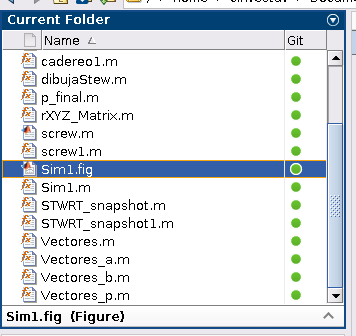
\includegraphics[scale=0.6]{img/GUI_start_click.PNG}
 \caption{Menú Current Folder.}
 \label{fig: start GUI}
\end{figure}


Para acceder al entorno GUIDE: 
\begin{itemize}
 \item  Seleccione el archivo \textbf{Sim1.fig} y haga clic secundario para 
acceder a las opciones del archivo. 
\item Elija la opción \textbf{Abrir en GUIDE}. 
MATLAB inicializará el entorno GUIDE inmediatamente. 
\item Desde la ventana mostrada en la 
figura \ref{fig: GUIDE} seleccione el menú 
\textbf{Herramientas} y oprima la opción \textbf{ejecutar}.
La interfaz gráfica será inicializada con los valores
precargados en el código fuente.
\end{itemize}


\begin{figure}[h]
 \centering
 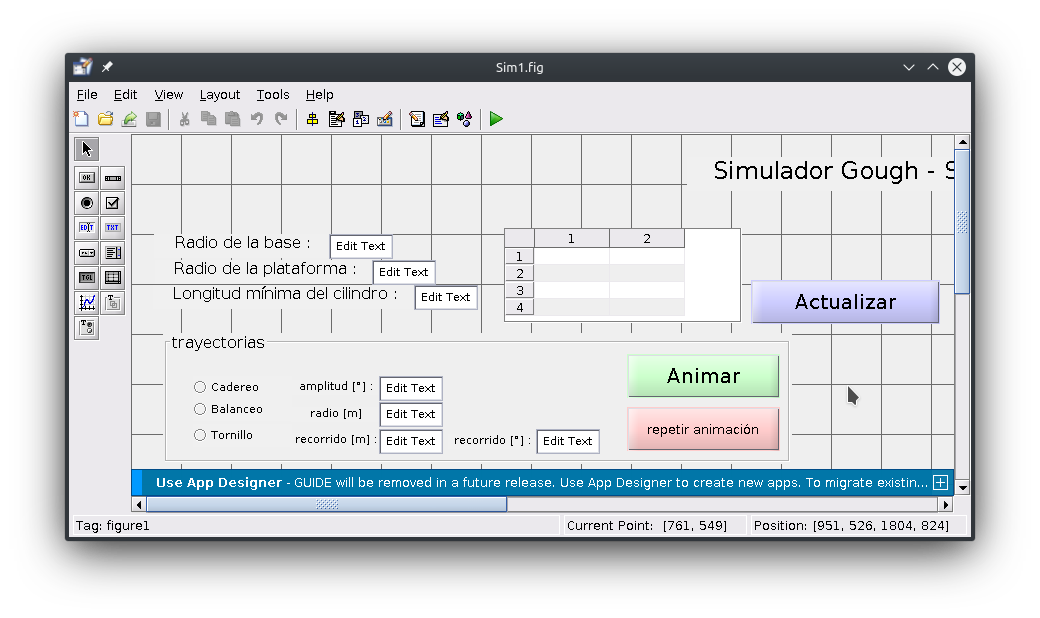
\includegraphics[scale=0.4]{img/GUI_GUIDE_window.PNG}
 \caption{Entorno GUIDE.}
 \label{fig: GUIDE}
\end{figure}


Para iniciar la interfaz gráfica sin los valores 
precargados, haga doble clic en el archivo desde la 
ventana de \textbf{Current Folder}.


% \pagebreak
% \section{Guía de uso}
% 
% La interfaz gráfica del paquete GSP está diseñada para
% permitir al usuario evaluar la factibilidad de 
% alcanzar la posición deseada del robot de acuerdo a 
% las limitaciones del sistema. 
% Con la interfaz es posible realizar lo siguiente:
% \begin{itemize}
%  \item Actualizar los parámetros del simulador para que
%  concuerden con los valores del robot real.
%  \item Especificar la posición deseada y su orientación.
%  \item Validar la factibilidad del movimiento.
%  \item Visualizar tres animaciones precargadas de movimientos.
% \end{itemize}

\section{Partes de la interfaz}

\begin{figure}[ht]
 \centering
 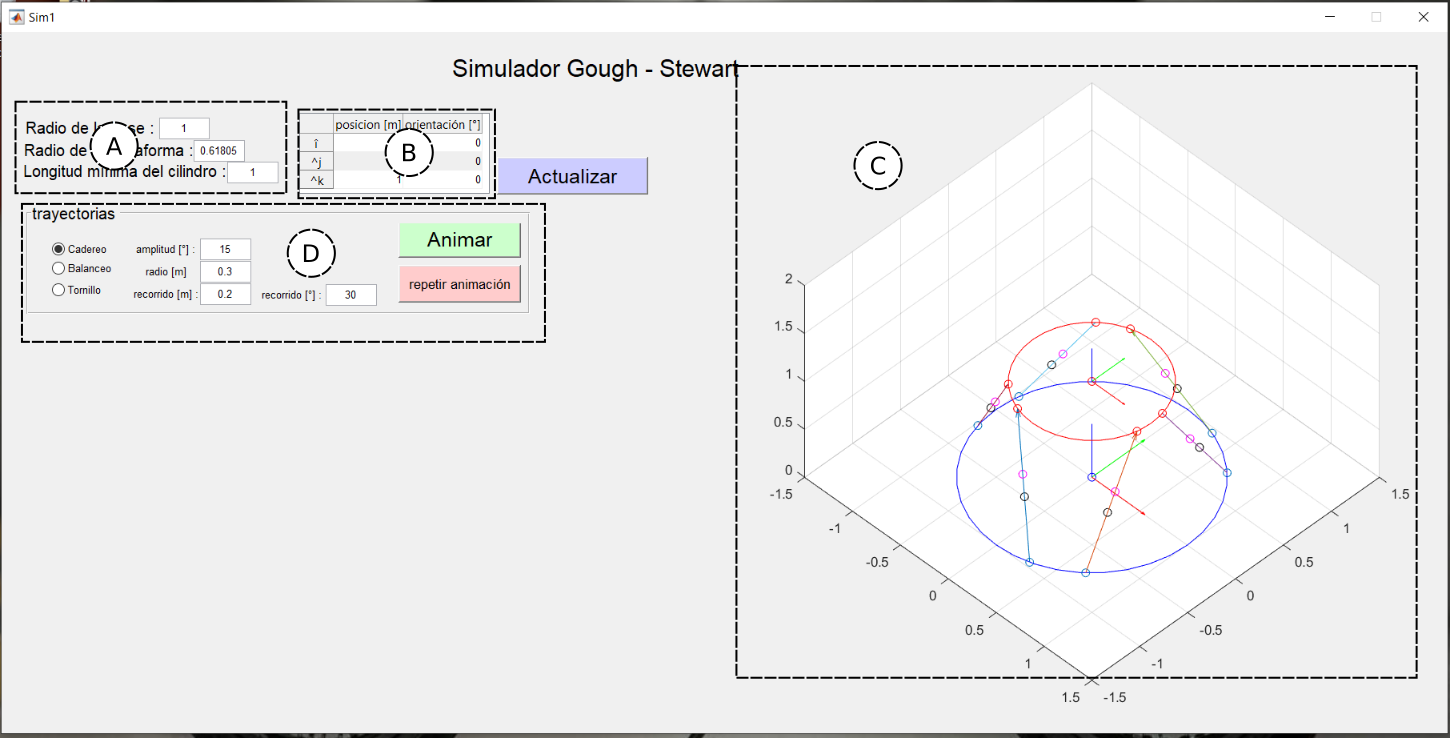
\includegraphics[scale=0.3]{img/gui_labels.PNG}
 \caption{Elementos de la interfaz gráfica.}
 \label{fig: GUI explained}
\end{figure}

\subsection{Parámetros de la plataforma}
El cuadro \textbf{A} de la figura 
\ref{fig: GUI explained} señala las tres cajas de entrada
de datos. El usuario puede actualizar estos valores a su conveniencia.


\subsection{Tabla de posicionamiento}
Contenida en el cuadro \textbf{B} de la figura \ref{fig: GUI explained}.
La posición y orientación deseadas pueden ser especificadas aquí.


\subsection{Validación}
El botón \textbf{Validar} es empleado para evaluar la factibilidad del
movimiento. 
Si es posible, el cuadro \textbf{C} será actualizado. 
De lo contrario arrojará un mensaje de error al usuario. 
Vea el capítulo \ref{chapter: troubleshooting} para más información.

\subsection{Animación}
Los controles incluidos en el cuadro \textbf{D} detallan las
opciones para generar animaciones basado en los parámetros del robot
y la posición deseada.



\section{Caso ejemplo}
La interfaz gráfica ya incluye un conjunto de 
demostraciones precargadas en la interfaz. 
Estas pueden ser accesadas al inicializar la interfaz
mediante el entorno GUIDE.

El robot está precargado con la siguiente 
configuración mostrada en la trabla \ref{tab: example}.
Accionand el botón \textbf{Actualizar}, los valores 
serán cargados en el simulador y el usuario 
podrá inicializar las animaciones disponibles en el paquete.

\begin{table}[h]
\begin{center}
\begin{tabular}{llcccc}
 & & Posición & & Orientación & \\
Radio de la base & 1 m. &  [x] & 0 m. &  [x] & 0\\
Radio de la plataforma & 0.61805 m. &  [y] & 0 m. &  [y] & 0\\
Longitud mínima del cilindro & 1 m. &  [z] & 1 m. &  [z] & 0
\end{tabular}
\end{center}
\caption{Parámetros del caso ejemplo.}
\label{tab: example}
\end{table}






